\documentclass{beamer}

\usepackage{tikz}
\usetikzlibrary{positioning,arrows,calc,fit,arrows.meta}
\tikzset{
	modal/.style={>=stealth,shorten >=1pt,shorten <=1pt,auto,node distance=1.5cm,
		semithick},
	world/.style={circle,draw,minimum size=0.5cm,fill=gray!15},
	point/.style={circle,draw,inner sep=0.5mm,fill=black},
	reflexive above/.style={->,loop,looseness=7,in=120,out=60},
	reflexive below/.style={->,loop,looseness=7,in=240,out=300},
	reflexive left/.style={->,loop,looseness=7,in=150,out=210},
	reflexive right/.style={->,loop,looseness=7,in=30,out=330}
}

\usepackage{xcolor}

\usepackage{amsmath, amssymb, amsthm}
\newcommand{\indep}{\mbox{$\perp\!\!\!\perp$}}
\newcommand{\notindep}{\mbox{ $\not\!\perp\!\!\!\perp$}}

\usepackage{graphics}

\setbeamertemplate{footline}[frame number]
\beamertemplatenavigationsymbolsempty


\begin{document}
	
\title{Causal Graphs }
\author{Julian Schuessler}
\date{November 5, 2019} 
\institute{Presentation for MZES Methods Bites}


\begin{frame}
	\titlepage
\end{frame}


\begin{frame}[t]
	\frametitle{Today}
	\tableofcontents
\end{frame}

\section{Love \& Mercy}

\begin{frame}[t]
\sectionpage
\end{frame}

\begin{frame}[t]
\frametitle{Love \& Mercy}
\begin{itemize}
	\item<2-> ``The 'insights' offered by the graphical approach to causal inference
	are generally not helpful'' (Donald Rubin)
	\item<3-> ``There are a lot of people who never use graphs, who are well-known in causal inference, who use this to the extent that they say we shouldn't use graphs. A famous saying in science is: Science progresses on the deaths of the older scientists. And I don't think graphs will have any trouble in the future.'' (James Robins)
	\item<4-> ``The DAG approach fully deserves the attention of all researchers and users of causal
	inference as one of its leading methodologies.'' (Guido Imbens)
	\item<5-> ``Knowledge of causal graphical models is a plus'' (job ad by Facebook)
\end{itemize}
\end{frame}

\section{Survey and Overview}

\begin{frame}[t]
\sectionpage
\end{frame}


\begin{frame}
\frametitle{Survey}
\begin{itemize}
	\item<1-> How would you rate your knowledge in potential outcomes / counterfactuals?
	\begin{itemize}
		\item<2-> Very good
		\item<2-> Good
		\item<2-> Ok
		\item<2-> A bit
		\item<2-> Nada
	\end{itemize}
	\item<2-> How would you rate your knowledge in causal graphs?
\begin{itemize}
	\item<3-> Very good
	\item<3-> Good
	\item<3-> Ok
	\item<3-> A bit
	\item<3-> Nada
\end{itemize}
\end{itemize}
\end{frame}

\begin{frame}
\frametitle{Survey: Structural Equations}
\begin{itemize}
	\item<1-> $Y = X\beta + \epsilon$. When does $\beta$ stand for the causal effect of $X$ on $Y$?
	\begin{itemize}
	\item<2-> Never
	\item<3-> If a researcher says so, and then w/o further assumptions
	\item<4-> If $E[\epsilon|X] = 0$ (``exogeneity'')
	\end{itemize}
\end{itemize}
\end{frame}


\begin{frame}
\frametitle{Choosing Control Variables}
\begin{itemize}
	\item<1-> Suppose you are interested in effect of $X$ on $Y$
	\item<2-> You ponder statistical control for other variable $Z$
	\item<3-> A good rule for choosing whether to include $Z$ would have two properties:
	\begin{itemize}
		\item<4-> It tells you which $Z$ you must control for
		\item<5-> It never tells you to control for a $Z$ which actually introduces bias
	\end{itemize}
\end{itemize}
\end{frame}

\frametitle{Choosing Control Variables}
\begin{frame}
\frametitle{Choosing Control Variables}
\begin{itemize}
	\item<1-> What do you think are good rules for choosing control variables?
	\item<2-> Control for $Z$ if...
	\begin{itemize}
		\item<3-> $Z$ associated with $Y$
		\item<4-> $Z$ associated with $X$
		\item<5-> Unaffected by $X$ and associated with $X$ and $Y$ (K. Imai)
		\item<6-> affects $Y$
		\item<7-> $X \indep Y|Z$
		\item<8-> $X \indep Y(x)|Z$ 
	\end{itemize}
\end{itemize}
\end{frame}

\frametitle{Choosing Control Variables}
\begin{frame}
\frametitle{Choosing Control Variables}
\begin{itemize}
	\item<1-> \textit{All} of these rules violate the two requirements 
	\item<2-> Except for $X \indep Y(x)|Z$
	\item<3-> ``Conditional ignorability''
	\item<4-> ``Conditional on $Z$, the potential outcome of $Y$ when $X$ is set to $x$ is independent of $X$''
	\item<5-> Central assumption in potential outcomes framework
	\item<6-> Who is confident in understanding this assumption? 
\end{itemize}
\end{frame}

\begin{frame}[t]
\frametitle{Structural Causal Models}

\begin{itemize}
	%\item<1-> I will talk about DAGs as part of a more general framework: SCM
	\item<1-> SCM: Graphs are understood as structural equations, and define potential outcomes
\item<1-> Potential outcomes are an important, indispensable part of ``the DAG approach''
\item<1-> Every assumption in potential outcomes can be depicted using a graph
\item<2-> Contra Twitter, \textit{there is no formal difference. It is only about representation of the math, and how easy to understand it is}
\end{itemize}
\end{frame}

\begin{frame}[t]
\frametitle{Structural Causal Models}

\begin{itemize}
	\item<1-> Three main problems and tools: 
	\begin{itemize}
		\item<2-> Understanding independencies implied by graph
		\item<3-> Definition and identification of causal effects using graphical rules
		\item<4-> Structural Definition of Potential Outcomes / Counterfactuals
	\end{itemize}
\end{itemize}
\end{frame}

\section{Graph Basics and d-separation}


\begin{frame}[t]
\sectionpage
\end{frame}

\begin{frame}[t]
\frametitle{What are the Assumptions?}
\begin{figure}[ht]
	\centering
	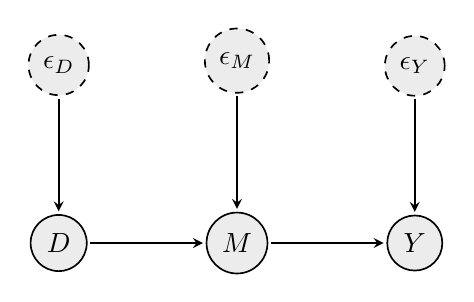
\begin{tikzpicture}[modal]
	
	\node[world] (d) {$D$};
	\node[world] (m) [right= of d] {$M$};
	\node[world] (y) [right= of m] {$Y$};
	\node[world, dashed] (ed) [above= of d] {$\epsilon_D$};
		\node[world, dashed] (em) [above= of m] {$\epsilon_M$};
			\node[world, dashed] (ey) [above= of y] {$\epsilon_Y$};
	
	\path[->] (d) edge (m);
	\path[->] (m) edge (y);
	\path[->] (ed) edge (d);
	\path[->] (em) edge (m);
	\path[->] (ey) edge (y);
	
	\end{tikzpicture}
\end{figure}
\begin{itemize}
	\item<1-> This is a directed acyclic graph (DAG)
	\item<1-> Which assumptions are depicted here?
	\item<2-> \textit{Absent} arrows: \begin{itemize}
		\item<3-> From $D$ to $Y$
		\item<4-> from $\epsilon_D$ to $M$ and $Y$, etc.
		\item<5-> from $M$ to $D$ and $Y$ to $M$ or $D$ (would make graph cyclic)
		\end{itemize}
	\item<6-> Sth. you have to learn: Look for arrows that aren't there
\end{itemize}
\end{frame}

\begin{frame}[t]
\frametitle{Exercise: IV Graph}
\color{blue}
	\huge
	 \begin{center}
 Exercise:
 \\

Draw ``the'' instrumental variables graph with \\
instrument $Z$ \\
 treatment $X$ \\
  outcome $Y$ \\
   unobserved confounder $U$
\end{center} 
\end{frame}

\begin{frame}[t]
\frametitle{The IV Graph}
\begin{figure}

	\centering
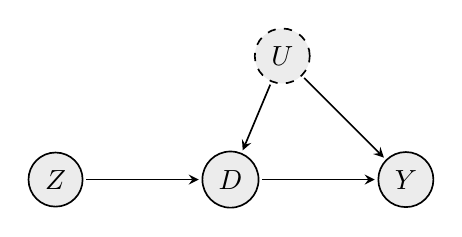
\begin{tikzpicture}[modal]

\node[world] (z) {$Z$};
\node[world] (d) [right= of z] {$D$};
\node[world] (y) [right= of d] {$Y$};
\node[world, dashed] (u) [above left= of y] {$U$};

\path[->] (z) edge (d);
\path[->] (d) edge (y);
\path[->] (u) edge (y);
\path[->] (u) edge (d);

\end{tikzpicture}
\end{figure}
\begin{itemize}
	\item<1-> Suppose you run a regression of $Y$ on $Z$ and $D$. Will the coefficient on $Z$ be zero?
	\item<2-> Discuss with your neighbor!
	\item<3-> We want to know whether a graph implies independencies between variables
	\item<4-> $\implies$ d-separation
\end{itemize}
\end{frame}

\begin{frame}[t]
\frametitle{d-separation I}
\begin{figure}[ht]
	\centering
	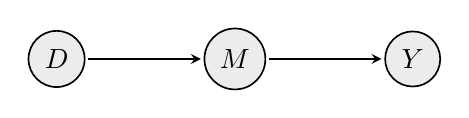
\begin{tikzpicture}[modal]
	
	\node[world] (d) {$D$};
	\node[world] (m) [right= of d] {$M$};
	\node[world] (y) [right= of m] {$Y$};
	%\node[world, dashed] (ed) [above= of d] {$\epsilon_D$};
	%\node[world, dashed] (em) [above= of m] {$\epsilon_M$};
	%\node[world, dashed] (ey) [above= of y] {$\epsilon_Y$};
	
	\path[->] (d) edge (m);
	\path[->] (m) edge (y);
	%\path[->] (ed) edge (d);
	%\path[->] (em) edge (m);
	%\path[->] (ey) edge (y);
	%\path[<->] (ed) edge[bend left = 15] (ey);
	\end{tikzpicture}
\end{figure}
\begin{itemize}
	\item<1-> In this graph, do $D$ and $Y$ correlate? 
	\begin{itemize}
		\item<2-> Yes
	\end{itemize}
\item<3-> Do $D$ and $Y$ correlate when I control for / condition on $M$?
\begin{itemize}
	\item<4-> No
\end{itemize}
\item<5-> The path is \textit{open}. Conditional on $M$, it is \textit{blocked}
\item<6-> Simulation in {\tt R}: \\
\pause[6] {\tt D <- rnorm(1000)} \\
{\tt M <- 0.4$*$D + rnorm(1000)} \\
 {\tt Y <- -0.6$*$M rnorm(1000) \\ 
 lm(Y $\sim$ D) \\
 lm(Y $\sim$ D + M)}
\end{itemize}
\end{frame}

\begin{frame}[t]
\frametitle{d-separation II}
\begin{figure}[ht]
	\centering
	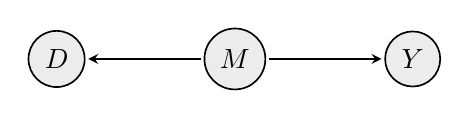
\begin{tikzpicture}[modal]
	
	\node[world] (d) {$D$};
	\node[world] (m) [right= of d] {$M$};
	\node[world] (y) [right= of m] {$Y$};
	%\node[world, dashed] (ed) [above= of d] {$\epsilon_D$};
	%\node[world, dashed] (em) [above= of m] {$\epsilon_M$};
	%\node[world, dashed] (ey) [above= of y] {$\epsilon_Y$};
	
	\path[->] (m) edge (d);
	\path[->] (m) edge (y);
	%\path[->] (ed) edge (d);
	%\path[->] (em) edge (m);
	%\path[->] (ey) edge (y);
	%\path[<->] (ed) edge[bend left = 15] (ey);
	\end{tikzpicture}
\end{figure}
\begin{itemize}
	\item<1-> In this graph, do $D$ and $Y$ correlate? 
	\begin{itemize}
		\item<2-> Yes
	\end{itemize}
	\item<3-> Do $D$ and $Y$ correlate when I control for / condition on $M$?
	\begin{itemize}
		\item<4-> No
	\end{itemize}
\item<5-> The path is \textit{open}. Conditional on $M$, it is \textit{blocked}
\end{itemize}
\end{frame}

\begin{frame}[t]
\frametitle{d-separation III}
\begin{figure}[ht]
	\centering
	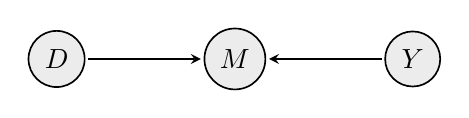
\begin{tikzpicture}[modal]
	
	\node[world] (d) {$D$};
	\node[world] (m) [right= of d] {$M$};
	\node[world] (y) [right= of m] {$Y$};
	%\node[world, dashed] (ed) [above= of d] {$\epsilon_D$};
	%\node[world, dashed] (em) [above= of m] {$\epsilon_M$};
	%\node[world, dashed] (ey) [above= of y] {$\epsilon_Y$};
	
	\path[->] (d) edge (m);
	\path[->] (y) edge (m);
	%\path[->] (ed) edge (d);
	%\path[->] (em) edge (m);
	%\path[->] (ey) edge (y);
	%\path[<->] (ed) edge[bend left = 15] (ey);
	\end{tikzpicture}
\end{figure}
\begin{itemize}
	\item<1-> In this graph, do $D$ and $Y$ correlate? 
	\begin{itemize}
		\item<2-> No
	\end{itemize}
	\item<3-> Do $D$ and $Y$ correlate when I control for / condition on $M$?
	\begin{itemize}
		\item<4-> Yes
	\end{itemize}
\item<5-> The path is \textit{blocked}. Conditional on $M$, it is \textit{open}
\item<6-> $M$ acts as a \textit{collider}
\end{itemize}
\end{frame}

\begin{frame}[t]
\frametitle{Collider: Example}
\begin{figure}[ht]
	\centering
	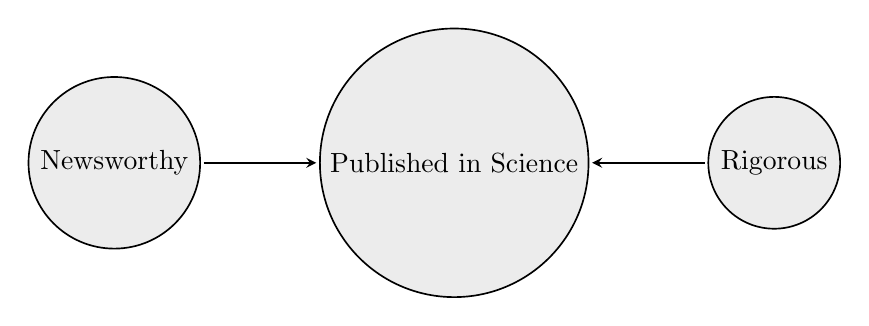
\begin{tikzpicture}[modal]
	
	\node[world] (d) {Newsworthy};
	\node[world] (m) [right= of d] {Published in Science};
	\node[world] (y) [right= of m] {Rigorous};
	%\node[world, dashed] (ed) [above= of d] {$\epsilon_D$};
	%\node[world, dashed] (em) [above= of m] {$\epsilon_M$};
	%\node[world, dashed] (ey) [above= of y] {$\epsilon_Y$};
	
	\path[->] (d) edge (m);
	\path[->] (y) edge (m);
	%\path[->] (ed) edge (d);
	%\path[->] (em) edge (m);
	%\path[->] (ey) edge (y);
	%\path[<->] (ed) edge[bend left = 15] (ey);
	\end{tikzpicture}
\end{figure}
\begin{itemize}
	\item<1-> If study is newsworthy and published in science...
	\item<2-> ... it is probably less rigorous
\end{itemize}
\end{frame}

\begin{frame}[t]
\frametitle{d-separation: Summary}

\begin{itemize}
	
	\item<1-> Chain of mediation: Path is open unconditionally, but blocked conditional on the middle node. $D \notindep Y$ but $D \indep Y|M$. 
	\item<2-> Common cause/fork: Path is open unconditionally, but blocked conditional on the middle node. $D \notindep Y$ but $D \indep Y|M$. 
	\item<3-> Collider: Path is blocked unconditionally, but open conditional on the middle node or one of its descendants. $D \indep Y$ but $D \notindep Y|M$. 
	\item<4-> What if there are multiple, longer paths between $D$ and $Y$? Will $D$ and $Y$ be (conditionally) independent? \textbf{d-separation} gives the answer
\end{itemize}
\end{frame}

\begin{frame}[t]
\frametitle{d-separation: Definition}

\begin{itemize}

\item<1-> A path p is blocked by a set of nodes $Z$ if and only if

1. p contains a chain of nodes $X \rightarrow M \rightarrow Y$ or a fork $X \leftarrow M \rightarrow Y$ such that the middle node $M$ is in $Z$ (i.e., $M$ is conditioned on), or

2. p contains a collider $X \rightarrow M \leftarrow Y$ such that the collision node $M$ is not in $Z$, and no descendant of $B$ is in $Z$
\item<2-> If $Z$ blocks every path between two nodes $X$ and $Y$, then $X$ and $Y$ are \textbf{d-separated}, conditional	on $Z$, and thus are independent conditional on $Z$
\item<3-> \textbf{testable implication} of the graph
\item<4-> ``d-separation'' = ``directional separation'' (in directed graphs)
\item<5-> Path p may be very long, but as long as you block sub-path, you block the whole path
\end{itemize}
\end{frame}

\begin{frame}[t]
\frametitle{The IV Graph}
\begin{figure}
	
	\centering
	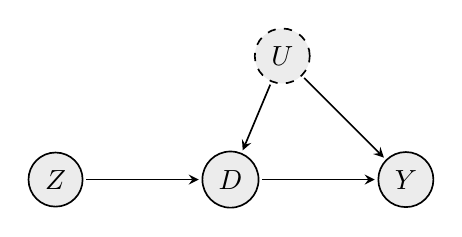
\begin{tikzpicture}[modal]
	
	\node[world] (z) {$Z$};
	\node[world] (d) [right= of z] {$D$};
	\node[world] (y) [right= of d] {$Y$};
	\node[world, dashed] (u) [above left= of y] {$U$};
	
	\path[->] (z) edge (d);
	\path[->] (d) edge (y);
	\path[->] (u) edge (y);
	\path[->] (u) edge (d);
	
	\end{tikzpicture}
\end{figure}
\begin{itemize}
	\item<1-> Suppose you run a regression of $Y$ on $Z$ and $D$. Will the coefficient on $Z$ be zero?
	\item<1-> Enumerate all paths between $Z$ and $Y$. Check whether there are any open paths, conditional on $D$
	\item<1-> Then check back with your neighbor
\end{itemize}
\end{frame}

\begin{frame}[t]
\frametitle{The IV Graph}
\begin{figure}
	
	\centering
	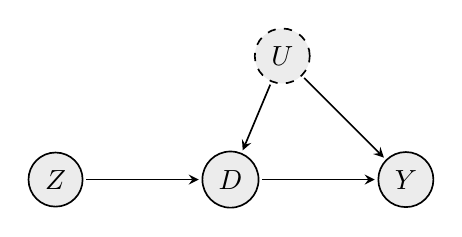
\begin{tikzpicture}[modal]
	
	\node[world] (z) {$Z$};
	\node[world] (d) [right= of z] {$D$};
	\node[world] (y) [right= of d] {$Y$};
	\node[world, dashed] (u) [above left= of y] {$U$};
	
	\path[->] (z) edge (d);
	\path[->] (d) edge (y);
	\path[->] (u) edge (y);
	\path[->] (u) edge (d);
	
	\end{tikzpicture}
\end{figure}
\begin{itemize}
	\item<1-> $Z \rightarrow D \rightarrow Y$
	\item<2-> $Z \rightarrow D \leftarrow U \rightarrow Y$
	\item<3-> First path is ``mediation'', blocked conditional on $D$
	\item<4-> Second path: $D$ is collider, open conditional on $D$
	\item<5-> $\implies$ In regression of $Y$ on $Z$ and $D$, coefficient of $Z$ will be non-zero
	\item<6-> Even though $Z$ is a valid IV, no direct effect
\end{itemize}
\end{frame}

\begin{frame}[t]
\frametitle{d-separation in Mediation Model}
	\begin{figure}[ht]
	\centering
	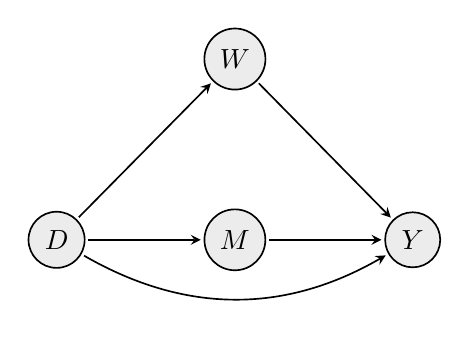
\begin{tikzpicture}[modal]
	
	\node[world] (d) {$D$};
	\node[world] (m) [right= of d] {$M$};
	\node[world] (y) [right= of m] {$Y$};
	\node[world] (w) [above= of m] {$W$};
	
	\path[->] (d) edge (m);
	\path[->] (d) edge (w);
	%\path[->] (w) edge (m);
	\path[->] (m) edge (y);
	\path[->] (d) edge[bend right] (y);
	\path[->] (w) edge (y);
	\end{tikzpicture}
\end{figure}
\begin{itemize}
	\item<1-> Does this graph have any testable implications? Check by inspecting whether any pair of variables are d-separated
	\item<2-> Hint: Variables that are directly connected can never be d-separated
	\item<3-> Work with your neighbor
\end{itemize}
\end{frame}

\begin{frame}[t]
\frametitle{d-separation in Mediation Model}
\begin{figure}[ht]
	\centering
	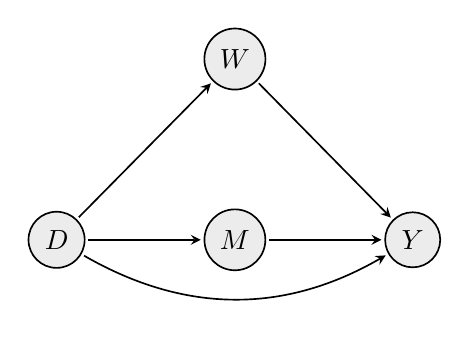
\begin{tikzpicture}[modal]
	
	\node[world] (d) {$D$};
	\node[world] (m) [right= of d] {$M$};
	\node[world] (y) [right= of m] {$Y$};
	\node[world] (w) [above= of m] {$W$};
	
	\path[->] (d) edge (m);
	\path[->] (d) edge (w);
	%\path[->] (w) edge (m);
	\path[->] (m) edge (y);
	\path[->] (d) edge[bend right] (y);
	\path[->] (w) edge (y);
	\end{tikzpicture}
\end{figure}
\begin{itemize}
	\item<1-> Only candidate pair: $M$ and $W$
	\item<2-> $W \leftarrow D \rightarrow M$
	\item<3-> $W \rightarrow Y \leftarrow M$
	\item<4-> $W \leftarrow D \rightarrow Y \leftarrow M$
	\item<5-> $\implies$ $W$ and $M$ d-separated conditional on $D$
\item<6-> Test, e.g.: Regress $W$ on $M$ and $D$. Which coefficient should be zero?
\item<7-> Coefficient on $M$
\item<8-> If not: misspecified regression / Type 1 error / graph wrong
\end{itemize}
\end{frame}

\section{Definition and Identification of Causal Effects}


\begin{frame}[t]
\sectionpage
\end{frame}

\begin{frame}[t]
\frametitle{Definition of Causal Effects}
\begin{figure}[ht]
	\centering
	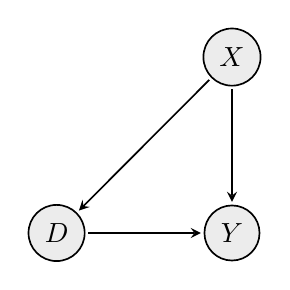
\begin{tikzpicture}[modal]
	
	\node[world] (d) {$D$};
	\node[world] (y) [right= of d] {$Y$};
	\node[world] (u) [above= of y] {$X$};
	
	\path[->] (d) edge (y);
	\path[->] (u) edge (y);
	\path[->] (u) edge (d);
	
	\end{tikzpicture}
\end{figure}
\begin{itemize}
	\item<1-> Hypothetical control of $D$ used to define causal effects
	\item<2-> How does the graph change if $D$ is set to $d$ externally?
	
	
\end{itemize}
\end{frame}

\begin{frame}[t]
\frametitle{Definition of Causal Effects}
\begin{figure}[ht]
	\centering
	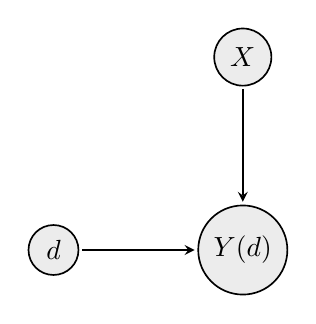
\begin{tikzpicture}[modal]
	
	\node[world] (d) {$d$};
	\node[world] (y) [right= of d] {$Y(d)$};
	\node[world] (u) [above= of y] {$X$};
	
	\path[->] (d) edge (y);
	\path[->] (u) edge (y);
	%\path[->] (u) edge (d);
	
	\end{tikzpicture}
\end{figure}
\begin{itemize}
	\item<1-> $E[Y|do(D = d)] = E[Y(d)]$
	
	
	
\end{itemize}
\end{frame}


\begin{frame}[t]
\frametitle{Intuition}
\begin{figure}[ht]
	\centering
	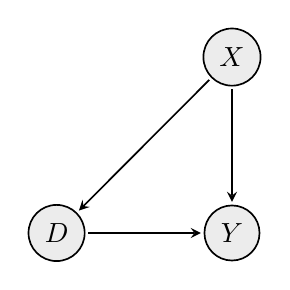
\begin{tikzpicture}[modal]
	
	\node[world] (d) {$D$};
	\node[world] (y) [right= of d] {$Y$};
	\node[world] (u) [above= of y] {$X$};
	
	\path[->] (d) edge (y);
	\path[->] (u) edge (y);
	\path[->] (u) edge (d);
	
	\end{tikzpicture}
\end{figure}
\begin{itemize}
	\item<2-> Which paths does the association between $D$ and $Y$ consist of?
	\item<3-> 1) causal effect of $D$ on $Y$ and  \visible<4->{2) confounding due to $X$}
	\item<5-> We want to estimate $E[Y|do(D = d)]$
	\item<6-> If you cannot $do(d)$ in reality, find control variables such that
	\begin{itemize}
		\item<6-> ``Bad'', ``spurious'', ``non-causal'' paths between $D$ and $Y$ are blocked
		\item<7-> All ``causal'' paths are left open
		\item<8-> No new ``non-causal'' paths are opened up (colliders...)
	\end{itemize}
	
	
	
\end{itemize}
\end{frame}

\begin{frame}[t]
\frametitle{Intuition}
\begin{figure}[ht]
\centering
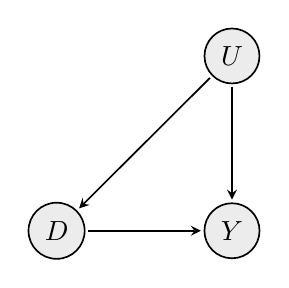
\begin{tikzpicture}[modal]

\node[world] (d) {$D$};
\node[world] (y) [right= of d] {$Y$};
\node[world] (u) [above= of y] {$U$};

\path[->] (d) edge (y);
\path[->] (u) edge (y);
\path[->] (u) edge (d);

\end{tikzpicture}
\end{figure}
\begin{itemize}
\item<1-> If you cannot intervene, find control variables such that
\begin{itemize}
	\item<1-> ``Bad'', ``spurious'', ``non-causal'' paths between $D$ and $Y$ are blocked
	\item<1-> All ``causal'' paths are left open
	\item<1-> No new ``non-causal'' paths are opened up (colliders...)
\end{itemize}
\item<2-> This is UNRELATED to d-separation: d-separation is for testing graphs; and if two variables are d-separated, by definition all paths between them are blocked
\item<3-> But for identifying causal effects, we certainly want to leave certain paths open (although we also want to block \textit{some})

\end{itemize}
\end{frame}

\begin{frame}[t]
\frametitle{The Back-Door Criterion}

\begin{itemize}
\item<1-> Given an ordered pair of variables $(D, Y)$ in a DAG $G$, a set of variables $X$ satisfies the backdoor criterion relative to $(D, Y)$ if 
\begin{center}
1) no node in $X$ is a descendant of $D$, and 

2) $X$ blocks every path between $D$ and $Y$ that contains an arrow into $D$, or: $X$ d-separates $D$ from $Y$ in $G_{\underline{D}}$ 
\end{center}
\vspace{1cm} 
\item<2-> \textit{Ordered} pair because $D$ is cause, $Y$ is effect 
%\item<3-> $X$ may satisfy BDC for $(D_1, Y)$ but not $(D_2, Y)$
\item<3-> A path that starts with an arrow into $D$ is called a \textbf{back-door path}
\item<4-> Blocking back-door paths makes sure we block ``bad'' paths
\item<5-> Not conditioning on descendants of $D$ makes sure we leave all ``good'' causal paths open and that we do not open up new bad paths
\item<6-> Holds for any DAG $\implies$ non-parametric, distribution-free 
\end{itemize}
\end{frame}

\section{Post-Treatment Bias}

\begin{frame}[t]
\sectionpage
\end{frame}

\begin{frame}[t]
\frametitle{Post-Treatment Variables: Problem 1}
\begin{figure}[ht]
\centering
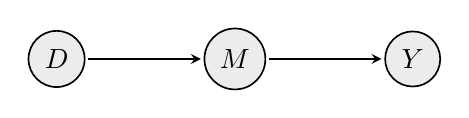
\begin{tikzpicture}[modal]

\node[world] (d) {$D$};
\node[world] (m) [right= of d] {$M$};
\node[world] (y) [right= of m] {$Y$};


\path[->] (d) edge (m);
\path[->] (m) edge (y);

\end{tikzpicture}
\end{figure}
\begin{itemize}
\item<1-> Which set of variables in this graph satisfy the BDC wrt effect of $D$ on $Y$?
\item<2-> The empty set $\emptyset$ - no controls necessary
\item<3-> $E[Y|do(D = 1)]- E[Y|do(D = 0) = E[Y|D = 1]- E[Y|D = 0]$ (correlation is causation)
\item<4-> No paths into $D$ - just like we intervened on it
\item<5-> Does $M$ correlate with $D$ and $Y$?
\item<6-> ``$M$ correlates with $D$ and $Y$. I've learned in stats that I need to control for it. Otherwise, I have omitted-variable bias''
\item<7-> Bad idea: Conditional on $M$, $D$ and $Y$ are d-separated! Even though $D$ may have an effect on $Y$
\item<8-> Montgomery et al. 2018 AJPS estimate that 50 \% of political science experiments do this. Huge problem.
\end{itemize}
\end{frame}

\begin{frame}[t]
\frametitle{Post-Treatment Variables: Problem 2}
\begin{figure}[ht]
\centering
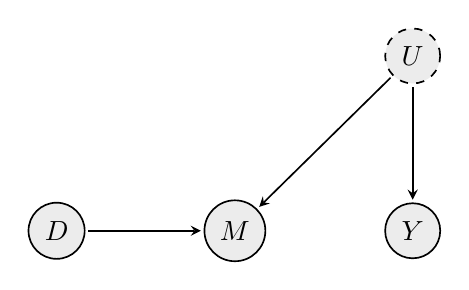
\begin{tikzpicture}[modal]

\node[world] (d) {$D$};
\node[world] (m) [right= of d] {$M$};
\node[world] (y) [right= of m] {$Y$};
\node[world, dashed] (u) [above= of y] {$U$};

\path[->] (d) edge (m);
\path[->] (u) edge (m);
\path[->] (u) edge (y);

\end{tikzpicture}
\end{figure}
\begin{itemize}
\item<1-> It gets worse. \visible<2->{Which set of variables in this graph satisfy the BDC wrt effect of $D$ on $Y$?}
\item<3-> The empty set - no controls necessary
\item<4-> $E[Y|do(D = 1)]- E[Y|do(D = 0)] = E[Y|D = 1]- E[Y|D = 0]$. What is $E[Y|D]$?
\item<5-> $E[Y|D] = E[Y]$ by d-separation. Correct estimator equals $E[Y] - E[Y] = 0$. Which is also clear from the graph.
\end{itemize}
\end{frame}

\begin{frame}[t]
\frametitle{Post-Treatment Variables: Problem 2}
\begin{figure}[ht]
\centering
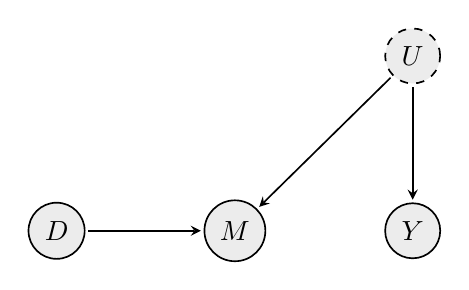
\begin{tikzpicture}[modal]

\node[world] (d) {$D$};
\node[world] (m) [right= of d] {$M$};
\node[world] (y) [right= of m] {$Y$};
\node[world, dashed] (u) [above= of y] {$U$};

\path[->] (d) edge (m);
\path[->] (u) edge (m);
\path[->] (u) edge (y);

\end{tikzpicture}
\end{figure}
\begin{itemize}
\item<1-> ``$M$ correlates with $D$ and $Y$. I've learned in stats that I need to control for it. Otherwise, I have omitted-variable bias''
\item<2-> Bad idea: Conditional on $M$, $D$ and $Y$ are d-connected! Collider!
\item<3-> $E[Y|D = 1, M = m] \neq E[Y|D = 1]$
\end{itemize}
\end{frame}

\begin{frame}[t]
\frametitle{Post-Treatment Variables: General Case}
\begin{figure}[ht]
\centering
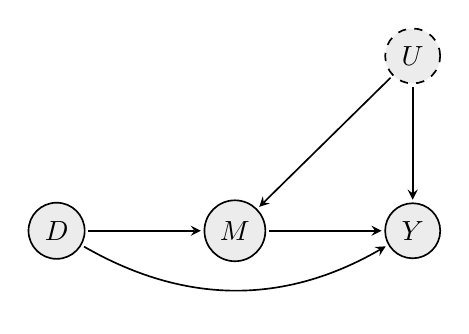
\begin{tikzpicture}[modal]

\node[world] (d) {$D$};
\node[world] (m) [right= of d] {$M$};
\node[world] (y) [right= of m] {$Y$};
\node[world, dashed] (u) [above= of y] {$U$};

\path[->] (d) edge (m);
\path[->] (u) edge (m);
\path[->] (u) edge (y);
\path[->] (m) edge (y);
\path[->] (d) edge[bend right] (y);
\end{tikzpicture}
\end{figure}
\begin{itemize}
\item<1-> This graph applies to situations where there are no back-door paths into $D$. Perhaps via randomization, or you block them by conditioning on $X$ (not shown).
\item<2-> Conditioning on $M$ is forbidden by the BDC and will have two consequences:
\item<3-> 1. You block a causal path, which you do not want
\item<4-> 2. You open up a non-causal path, which you do not want
\item<5-> This introduces bias, and it can go in any direction 
\end{itemize}
\end{frame}

\begin{frame}[t]
\frametitle{Post-Treatment Variables: Remarks}
\begin{itemize}
\item<1-> Although it is intuitively clear using causal graphs, the fact that conditioning on the descendants of the treatment may actually introduce bias is not well-known
\item<2-> Usually not mentioned in textbooks that do not use causal graphs
\item<3-> Even if mentioned, not really explained (see for example ``Mostly Harmless Econometrics'', section on ``Bad Control'') 
\end{itemize}
\end{frame}

\section{Causal Mediation}

\begin{frame}[t]
\sectionpage
\end{frame}

\begin{frame}[t]
\frametitle{Intuition for Natural Direct Effects}
\begin{figure}[ht!]
	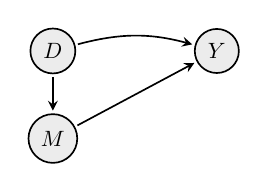
\begin{tikzpicture}[modal, scale=0.8, every node/.style={scale=0.8}]
	
	\node[world] (d) {$D$};
	\node[world] (y) [right= of d] {$Y$};
	\node[world] (m) [below=0.5cm of d] {$M$};
	
	
	\path[->] (d) edge (m);
	\path[->] (d) edge[bend left=15] (y);
	\path[->] (m) edge (y);
	
	
	\end{tikzpicture}
	

	
\end{figure}
\end{frame}

\begin{frame}[t]
\frametitle{Intuition for Natural Direct Effects}
\begin{figure}[ht!]
	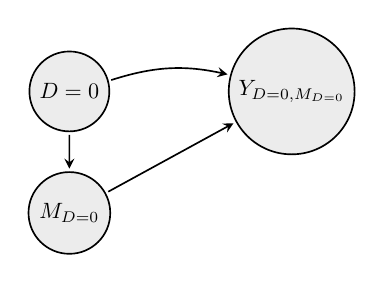
\begin{tikzpicture}[modal, scale=0.8, every node/.style={scale=0.8}]
	
	\node[world] (d) {$D = 0$};
	\node[world] (y) [right= of d] {$Y_{D = 0, M_{D = 0}}$};
	\node[world] (m) [below=0.5cm of d] {$M_{D = 0}$};
	
	
	\path[->] (d) edge (m);
	\path[->] (d) edge[bend left=15] (y);
	\path[->] (m) edge (y);
	
	
	\end{tikzpicture}
	
	(a) Set D = 0
	
	\visible<2->{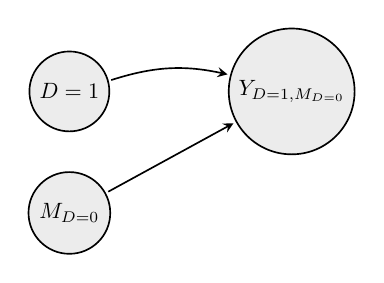
\begin{tikzpicture}[modal, scale=0.8, every node/.style={scale=0.8}]
		
		\node[world] (d) {$D = 1$};
		\node[world] (y) [right= of d] {$Y_{D = 1, M_{D = 0}}$};
		\node[world] (m) [below=0.5cm of d] {$M_{D = 0}$};
		
		
		\path[->] (d) edge[bend left=15] (y);
		\path[->] (m) edge (y);
		\end{tikzpicture}
		
		(b) Set D = 1, but disable D $\rightarrow$ M path}
	\begin{itemize}
		\item<3-> Note that $D$ is fixed while $M_{D = d}$ is random throughout! 
	\end{itemize}
	
\end{figure}
\end{frame}

\begin{frame}[t]
\frametitle{Definition of Natural Direct Effects}
\begin{columns}
\begin{column}{0.7\textwidth}
	\begin{itemize}
		\item<1-> First intervention gives $E[Y_{D = 0, M_{D = 0}}] = E[Y_{D = 0}]$
		\item<2-> Second intervention gives $E[Y_{D = 1, M_{D = 0}}]$
		\item<3-> Difference is $E[Y_{D = 1, M_{D = 0}}] - E[Y_{D = 0}] = NDE(0, 1)$
		\item<4-> The \textbf{natural direct effect} of changing $D$ from $0$ to $1$ while leaving mediator(s) $M$ as if $D = 0$
	\end{itemize}
\end{column}

\begin{column}{0.3\textwidth}
	\begin{figure}[ht!]
		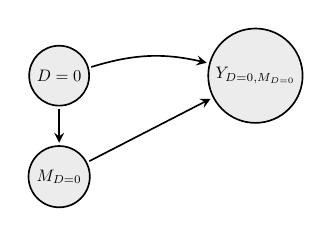
\begin{tikzpicture}[modal, scale=0.6, every node/.style={scale=0.6}]
		
		\node[world] (d) {$D = 0$};
		\node[world] (y) [right= of d] {$Y_{D = 0, M_{D = 0}}$};
		\node[world] (m) [below=0.5cm of d] {$M_{D = 0}$};
		
		
		\path[->] (d) edge (m);
		\path[->] (d) edge[bend left=15] (y);
		\path[->] (m) edge (y);
		
		
		\end{tikzpicture}
		
		(a) Set D = 0
		
		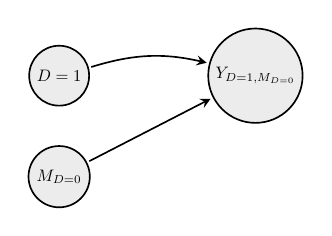
\begin{tikzpicture}[modal, scale=0.6, every node/.style={scale=0.6}]
		
		\node[world] (d) {$D = 1$};
		\node[world] (y) [right= of d] {$Y_{D = 1, M_{D = 0}}$};
		\node[world] (m) [below=0.5cm of d] {$M_{D = 0}$};
		
		
		\path[->] (d) edge[bend left=15] (y);
		\path[->] (m) edge (y);
		\end{tikzpicture}
		
		(b) Set D = 1, but disable D $\rightarrow$ M path
	\end{figure}
\end{column}
\end{columns}
\end{frame}


\begin{frame}[t]
\frametitle{Sequential Ignorability: Imai et al. 2010}
\begin{itemize}
	\item<1-> $D \indep M(d), Y(d', m)|X$
	\item<2-> $Y(d', m) \indep M(d')|X$
	\item<3-> or was it
		\item<4-> $D \indep M(d), Y(d', m)|X$
	\item<5-> $Y(d', m) \indep M(d')|D, X$
		\item<6-> or was it
	\item<7-> $D, M(d) \indep Y(d', m)|X$
	\item<8-> $Y(d', m) \indep M(d')|D, X$?
\end{itemize}
\end{frame}

\begin{frame}[t]
\frametitle{Sequential Ignorability: Graphical Version}
\begin{itemize}
	\item<1-> Graphical version of Sequential Ignorability (Imai et al. 2010) due to Pearl 2014:
	\item<1-> There are covariates $X$ such that 
	\item<2-> 1. $X$ and $D$ block all $D$-avoiding back-door paths from $M$ to $Y$	
	\item<2-> 2. $X$ blocks all back-door paths from $D$ to $M$ and from $D$ to $Y$, and no member of of $X$ is descendant of $D$
\end{itemize}
\end{frame}

\begin{frame}[t]
\frametitle{Comparison}
\begin{itemize}
	\item<1-> $D$ is jointly independent from potential outcome of $M$ when $D$ is set to $d$ and potential outcome of $Y$ when $D$ is set to $d'$ and $M$ is set to $m$, conditional on $X$
	\item<1-> The potential outcome of $Y$ when $D$ is set to $d$ and $M$ is set to $m$ is independent form the potential outcome of $M$ when $D$ is set to $d'$
	\item<2-> There are covariates $X$ such that 
	\item<2-> 1. $X$ and $D$ block all $D$-avoiding back-door paths from $M$ to $Y$	
	\item<2-> 2. $X$ blocks all back-door paths from $D$ to $M$ and from $D$ to $Y$, and no member of of $X$ is descendant of $D$
\end{itemize}
\end{frame}

\section*{Wrap-Up}
\begin{frame}[t]
\sectionpage
\end{frame}


\begin{frame}[t]
\frametitle{Wrap-Up}
\begin{itemize}
	\item<1-> Everyone interested in causal inference should learn about causal graphs
	\item<1-> Ideally, about structural causal models: Graphs plus structural equations plus potential outcomes
	\item<1-> Best textbook on the market: Pearl/Jewell/Glymour: Causal Inference. A Primer.
	\item<1-> Teaching material at \href{julianschuessler.net}{julianschuessler.net}
\end{itemize}
\end{frame}

\begin{frame}[t]
\frametitle{More stuff?}
\begin{itemize}
	\item<1-> Sample selection bias / generalizability
	\item<1-> Multiple interventions / controlled direct effects
	\item<1-> Panel Data
	\item<1-> More on IV 
	\item<1-> Sensitivity Analysis
\end{itemize}
\end{frame}

\end{document}